%\chapter{Les apports de la visualisation dans l'exploration d'un modèle}
%\label{chap:chap6}
%\begin{center}
%	{\large Version 2018-XX-XX}
%\end{center}
%\minitoc
%
%\section{Comment visualiser des données de simulation?}
%\subsection{Intégrer les données continuellement pour favoriser les allers-retours}
%\subsection{Visualisation et agrégation}
%\subsection{Quelle(s) agrégation(s) d'un espace théorique ?}
%\subsection{Visualiser les variations}
%
%\section{De la visualisation à l'exploration interactive}
%\subsection{Les apports des \textit{visual analytics} à la compréhension des données}
%\subsection{Rendre plus accessibles des données complexes et massives}
%\subsection{Pousser à la sérendipité par l'exploration interactive et intuitive}
%
%\section{Co-évolution du modèle et de ses interfaces d'exploration}
%\subsection{Adapter les outils aux demandes des utilisateurs}
%\subsection{Adapter les outils aux évolutions du modèle}
%\subsection{Comment comparer des modèles dotés d'indicateurs différents ?}


\chapter{Exploration du comportement de SimFeodal}
\label{chap:chap6}
\begin{center}
	{\large Version \hl{2019-08-20}}
\end{center}
\minitoc

\clearpage
\section*{Introduction}
\addcontentsline{toc}{section}{\protect\numberline{}Introduction}

Les chapitres précédents ont présenté le modèle SimFeodal (\hl{chapitre 2}), la manière de l'évaluer (\hl{chapitre 3}), la méthode suivie pour le paramétrage du modèle (\hl{chapitre 4}) et les outils développés pour mener à bien ces étapes de construction et d'évaluation (\hl{chapitre 5}).
Avec cet outillage, théorique, méthodologique et technique, nous sommes désormais en mesure d'explorer le modèle SimFeodal.
Par \og explorer le modèle\fg{}, on entend ici l'exploration des sorties produites par le modèle, sous toutes leurs formes, afin de gagner en connaissance sur ce qui est modélisé, mais aussi sur la manière dont le modèle est construit et implémenté.
Il s'agit autant d'analyser les \og résultats\fg{} de SimFeodal que d'en explorer le fonctionnement et la robustesse.
Ce chapitre est construit en trois parties, assez indépendantes les unes des autres, mais qui se concentrent sur différents aspects de l'évaluation d'un modèle.

La première partie concerne l'analyse des \og résultats\fg{} de SimFeodal, c'est-à-dire les réponses produites par le modèle aux questionnements énumérés dans le \hl{chapitre 3} :
le modèle aboutit-il bien à une polarisation des foyers paysans ?
Le système de peuplement généré par le modèle est-il hiérarchisé tel qu'on l'attendait, et sa distribution est-elle proche des connaissances empiriques ?
Observe-t-on une fixation du peuplement, dans un espace plus disséminé que dans les configurations initiales ?
Pour répondre à ces questions, on présente les étapes de calibrage qui ont permis d'aboutir à une version \og définitive\fg{} du modèle, ainsi que les éléments les plus marquants des indicateurs de sortie issus de cette version.

La deuxième partie de ce chapitre s'attachera à une exploration du comportement en lui-même, c'est-à-dire à sa sensibilité.
Cette sensibilité peut être entendue au sens de robustesse du modèle face aux différentes valeurs de paramètres (analyse de sensibilité classique).
Dans le cas de SimFeodal, une analyse de ce type pose toutefois des questions méthodologiques complexes, en raison notamment du grand nombre de paramètres impliqués et de \og l'explosion combinatoire\fg{} qui en découle.
Un autre perspective sur la sensibilité du modèle concerne sa robustesse face à l'aléa : dans quelle mesure les différents paramètres -- et leurs valeurs associées -- jouent-ils sur la variabilité des indicateurs de sortie ?

La dernière partie doit aussi permettre de gagner en compréhension du modèle en lui-même, et par cela de ce qui est modélisé.
Il s'agira d'explorer des \og scénarios\fg{}, c'est-à-dire de tester des hypothèses, sous la forme d'ensemble de valeurs de paramètres ayant un sens empirique, pour lesquelles le modèle n'a pas été calibré.
La réaction du modèle à ces scénarios sera l'occasion de comprendre plus profondément le comportement du modèle, mais aussi d'esquisser de premières pistes de réponses sur des questions empiriques que se posent les thématiciens spécialistes de la période étudiée.
Ces scénarios peuvent de plus concourir à l'évaluation du modèle.
Ils agissent comme des méthodes de \og validation croisée\fg{} qualitative : si le modèle donne des résultats satisfaisants sur des éléments pour lesquels il n'a pas été construit, cela contribue à renforcer la vraisemblance des postulats sur lesquels il est conçu.

\section{Calibrage du modèle et premiers résultats}

Dans le chapitre 3 (\cref{sec:evaluer-modele}), on indiquait que SimFeodal s'inscrivait dans la lignée des  modèles dont le but est d'\og assister la construction de théories\fg{}, ou encore \og à utilité de développement\fg{}, c'est-à-dire permettant à des chercheurs d'expliciter et de vérifier la cohérence de leurs hypothèses plutôt qu'à les infirmer ou confirmer.

En tant que tels, les \og résultats\fg{} de SimFeodal ne nous semblent donc pas revêtir d'enjeu confirmatoire majeur : ils sont là pour participer à l'évaluation du modèle, tant sur un plan interne qu'externe (cf. \hl{chap3}), mais ne constituent pas pour autant des éléments objectifs et quantifiables de validation.

Dans cette partie, nous rappelons les objectifs du modèle, nous décrivons les étapes de calibrage qui ont été nécessaires afin d'en approcher, et nous présentons enfin les résultats de la version actuelle (6.5.1) du modèle, c'est-à-dire les indicateurs de sortie de simulation issus de cette version, commentés selon la perspective de leur correspondance aux objectifs.

\subsection{Différencier objectifs contextuels et émergents}

\begin{tcolorbox}[breakable,left=0pt,right=0pt,top=0pt,bottom=0pt,
	colback=yellow!50,colframe=black,width=\dimexpr\textwidth\relax, 
	enlarge left by=0mm, boxsep=5pt,arc=0pt,outer arc=0pt]
\textbf{N.B.} : Toute cette partie 6.1.1 (et sans doute 6.1.2) serait bien plus logiquement située dans le chapitre 4 sur le paramétrage.
Il faudra notamment y mettre à jour la typologie des paramètres, et sans doute amener aussi le distinguo entre objectifs émergents et objectifs contextuels, qui en découle largement.
\end{tcolorbox}

Dans les chapitres précédents, on a présenté de manière extensive les objectifs -- dans tous les sens du terme -- poursuivis par le modèle.
Dans le chapitre \hl{2}, on décrivait l'objectif théorique du modèle, à savoir d'aider à la compréhension des phénomènes de restructuration spatiale du système de peuplement rural entre les IX$^e$ et XIII$^e$ siècles.
Dans le chapitre \hl{3}, on présentait la formalisation, au moyen d'indicateurs de sortie de simulation, des résultats du modèle.
En définissant un ensemble d'objectifs, qualifiés (allures de courbes, ordres de grandeur\ldots) sinon quantifiés (les indicateurs numériques), on esquissait un crible d'évaluation du modèle.

Pourtant, même au sein des indicateurs de sortie de simulation, il est une distinction que l'on n’a pas encore réalisée : le distinguo entre des indicateurs \og émergents\fg{} et des indicateurs \og contextuels\fg{}.

\begin{itemize}
	\item Les premiers sont les indicateurs les plus classiques en modélisation agent : on s'attache à leur évaluation parce qu'ils sont entièrement générés par la combinaison et l'intrication des mécanismes du modèle.
	Parvenir à obtenir des valeurs proches des connaissances empiriques dans ces modèles est un critère de validation d'un modèle, et donc potentiellement un signe d'acquisition de connaissance thématique ou théorique.
	Par exemple, dans SimFeodal, le taux de foyers paysans dispersés en fin de simulation est un pur indicateur émergent : le modèle n'a nullement été paramétré ou calibré pour lui faire atteindre une certaine valeur, et le taux obtenu donne des éléments d'interprétation thématique sur le modèle.
	\item Les indicateurs contextuels n'apportent aucune connaissance thématique.
	Ils remplissent un rôle de cadrage pour les indicateurs émergents : le modèle est paramétré et calibré pour que ces indicateurs parviennent à un résultat pré-décidé.
	Le calibrage des paramètres associés (c'est-à-dire des paramètres qui ont un impact majeur sur ces indicateurs) permet donc d'obtenir un contexte dans lequel les indicateurs émergents pourront être exploités.
	Pour illustrer ces indicateurs de contexte, on peut prendre l'exemple, dans SimFeodal, du nombre de foyers paysans en fin de simulation : ce nombre est entièrement dépendant de deux paramètres (quantité initiale et taux de croissance), et constitue donc presque un \textit{input}, c'est-à-dire ici un contexte au sein duquel les autres indicateurs s'exprimeront.
\end{itemize}

Le tableau des objectifs présent dans SimEDB (\hl{figure 5.8} du \hl{chapitre 5}) correspond à une partie des indicateurs de sortie (les indicateurs numériques ici) de ces deux types, tel qu'indiqué dans le \cref{tab:objectifs-types}.

\begin{table}[H]
	\captionsetup{singlelinecheck=off}
	\centering
	\small
	{\renewcommand{\arraystretch}{1.3}%
	\begin{tabular}{|p{4.5cm}|p{2.1cm}|p{1.9cm}|p{4.5cm}|}
		\hline
		\textbf{Indicateur} & \textbf{Valeur attendue}\footnotemark & \textbf{Type} & \textbf{Dépendances directes}\footnotemark \\ \hline
		\textit{Agrégats} & \textit{200} & Émergent & \multicolumn{1}{c|}{--} \\ \hline
		\rowcolor[HTML]{DCDCDC} \textit{Châteaux} & \textit{50} & Contextuel & probabilités de construction de châteaux (PS et GS) \\ \hline
		\textit{Gros châteaux} & \textit{10} & Émergent & \multicolumn{1}{c|}{--} \\ \hline
		\rowcolor[HTML]{DCDCDC} \textit{Seigneurs} & \textit{200} & Contextuel & paramètre~dédié~: (\textsf{objectif\_nombre\_seigneurs}) \\ \hline
		\textit{Églises paroissiales} & \textit{300} & Émergent & \multicolumn{1}{c|}{--} \\ \hline
		\textit{Distance moyenne entre églises} & \textit{3 000 m} & Émergent & \multicolumn{1}{c|}{--} \\ \hline
		\textit{Part de foyers paysans isolés} & \textit{20 \%} & Émergent & \multicolumn{1}{c|}{--} \\ \hline
		\textit{Augmentation de la charge fiscale des foyers paysans} & \textit{x 3} & Émergent & \multicolumn{1}{c|}{--} \\ \hline
		\rowcolor[HTML]{DCDCDC} \textit{Nombre de Foyers Paysans} & 50 000 & Contextuel & nombre initial; taux de croissance\\ \hline
		\rowcolor[HTML]{DCDCDC} \textit{Densité de population} & 8 feux/km² & Contextuel & nombre de foyers paysans ; taille du monde \\ \hline
	\end{tabular}}
	\caption{Les objectifs numériques, contextuels et émergents, de SimFeodal.}
	\label{tab:objectifs-types}
\end{table}
\footnotetext{Objectif en fin de simulation.}
\footnotetext{Paramètres influant directement sur la valeur de l'indicateur.}

Notons que si ces indicateurs ont une cohérence à être présentés ensemble au sein de SimEDB, dans le cas d'un tableau de synthèse dédié à l'exploration des résultats de simulation, leur traitement doit nécessairement être différent en matière d'évaluation du modèle.
Cette distinction nous paraît importante en vue d'aborder le calibrage du modèle.
En effet, étant donné la large quantité de paramètres dans le modèle, dont une combinaison judicieuse peut certainement aboutir à des résultats diamétralement opposés, il était nécessaire de restreindre le nombre de paramètres sur lesquels agir pour calibrer le modèle.
Pour que ce calibrage ne soit pas guidé par une logique tautologique, en contraignant le modèle à produire des résultats attendus, on a choisi de mener le calibrage sur les éléments de contexte et sur les éléments techniques (cf. la typologie du \hl{chapitre 4.}\footnote{
	\hl{Le chapitre 4 est à reprendre, notamment en supprimant la typologie des paramètres commensurables, techniques etc. et en la remplaçant par la typologie utilisée dans le modèle, cf. tableau des paramètres : inputs, paramètres de contexte, paramètres de mécanismes, paramètres techniques.}
}
).

\subsection{Calibrage du modèle}

La phase de calibrage diffère des nombreuses étapes de paramétrage décrites dans le \hl{chapitre 4}.
Il  ne s'agit ainsi plus d'ajuster les mécanismes et paramètres pour obtenir une cohérence d'ensemble plus importante dans la manière dont le modèle réagit, mais de se concentrer sur quelques paramètres et indicateurs de sortie\footnote{
Conceptuellement, paramètres et indicateurs sont très largement différents, situés de part et d'autre de la simulation dans une typologie comme celle de Balci (ref chap 4).
Pourtant, dans le cas de ces éléments de contexte, les paramètres sont étroitement liés, de manière presque déterministe, aux indicateurs de sortie qui en découleront.
Pour \og ajuster\fg{} la valeur d'un indicateur de sortie, on pourra donc tester différents ensembles de valeurs pour le ou les paramètres qui agissent directement sur ces indicateurs.
}, contextuels, dont on va régler finement les valeurs de paramètre afin que le contexte de déroulement des autres mécanismes du modèle soit aussi contrôlé et fidèle aux connaissances expertes que possible.

Le calibrage d'un paramètre peut résulter d'un ajustement issu de simulations, par exemple en trouvant de manière expérimentale une valeur de paramètre qui assurera un écart minimal entre l'indicateur de sortie de simulation visé et sa correspondance empirique.
Le calibrage peut aussi être thématique, par exemple en menant une recherche plus approfondie sur les valeurs que peuvent prendre, thématiquement, certains paramètres du modèle au regard des connaissances expertes sur lesquels ils s'appuient.
Ce second type de calibrage pourrait sembler évident, préalable à une démarche rigoureuse et scientifique, et indispensable à réaliser sur chacun des paramètres d'un modèle, ce qui est d'ailleurs vraisemblablement fait dans la plupart des modèles.
Dans un modèle descriptif, exploratoire et surtout basé sur des dynamiques passées, pourtant, la tâche de recherche précise de valeurs pour des dizaines de paramètres semble irréalisable en dehors de projets de modélisation de très large ampleur, ce qui n'est pas le cas de SimFeodal.

Dans les paragraphes suivant, nous donnons des exemples de paramètres et indicateurs qui ont été calibrées dans les dernières phases de paramétrage du modèle.
Ces exemples reprennent la distinction établie ci-dessus entre les types de calibrages : le calibrage des \textit{inputs} est entièrement thématique, celui des paroisses est mixte, entre thématique et expérimental, et le calibrage des châteaux est purement expérimental, guidé par un objectif thématique pré-défini clair.


\subsubsection*{Inputs}
\paragraph{Taille du monde}

Depuis sa conception (en 2014) jusqu'à la version 5.1 (Novembre 2018) du modèle, on avait choisi de simuler les agents du modèle dans un monde théorique, de forme carrée, de 100 km de côté.
Ces dimensions donnaient au monde l'étendue des grands départements français contemporains (ou des petites régions), et constituaient ainsi l'échelle à laquelle on souhaitait modéliser les phénomènes décrits dans SimFeodal.
Les différentes quantités empiriques relatives à cette dimension y étaient donc fortement liées : population, quantité d'églises, de petites villes etc.
On s'appuyait sur l'exemple de la Touraine historique, mais sans hésiter à inclure quelques éléments du duché d'Anjou voisin s'ils avaient été, à un moment ou à un autre, intégrés à notre région d'étude.

En faisant le choix de caler les dimensions du monde simulé plus fortement sur celles de la Touraine historique, il a fallu en premier lieu revoir à la baisse la taille du monde simulé.
La Touraine historique a ainsi une superficie proche de de 6 200 km², qui est ainsi inférieure de plus d'un tiers à la superficie originellement choisie ($100 \times 100$ km, soit 10 000 km²).
On a donc choisi, pour conserver un aspect carré et théorique, de diminuer la taille des côtés du monde simulé à 80 km, dont seuls 79 sont utilisables dans le cadre du modèle (voir le monde restreint, \hl{chapitre 2}), soit une surface de 6 240 km², équivalente à celle de la Touraine.

Dans SimFeodal, la plupart des mécanismes ont une importante composante spatiale.
Dès lors, avec la diminution de la superficie du monde, il a été nécessaire de modifier une large partie des paramètres techniques et certains paramètres de contexte.
Par exemple, un paramètre technique (\textsf{coef\_redevance}) permet d'ajuster le seuil de satisfaction matérielle des foyers paysans en fonction du nombre de redevances dont ils doivent s'acquitter.
En diminuant la taille du monde, et sans diminuer proportionnellement le nombre ou les surfaces des zones de prélèvement, le nombre de redevances des foyers paysans augmente mécaniquement.

\paragraph{Population}
Le nombre de foyers paysans aurait aussi pu être affecté par la taille du monde, mais on le considère comme un \textit{input} guidé par les connaissances empiriques plus que comme un élément contextuel.
Il nous faut ici pondérer fortement ce recours aux connaissances empiriques : il est extrêmement difficile, sinon vain, de parvenir à une simple estimation de la population d'une région française durant la période étudiée.
On peut avoir des indices sur des ordres de grandeur de population à des moments clés de l'histoire, mais d'une part, ils sont extrêmement incertains, et d'autre part, ces moments clés sont souvent différents des seuils temporels sur lesquels nous nous basons.
Sur la Touraine, l'expertise des archéologues et historiens (ref à EZR + Monique Bourrin) permet par exemple d'avoir une idée de la population au début du XVII$^e$ siècle, mais les différentes sources préalables présentent des écarts majeurs.

Pour SimFeodal, on a repris une hypothèse d'historien, qui semble ne pas faire trop débat dans la communauté.
Cette hypothèse consiste à penser qu'un optimum démographique a été atteint au début du XIII$^e$ siècle, et que la population a alors diminué considérablement.
Les historiens estiment que les populations du XIII$^e$ siècle n'ont été rattrapées qu'au début du XVII$^e$.
Il serait donc possible de considérer les populations à l'issu de la période étudiée comme proches de celles, mieux connues empiriquement, du XVII$^e$ siècle.
On a donc choisit de fixer un objectif de population, en fin de simulation (en 1200), à 50 000 foyers paysans, soit une densité d'environ 8 feu / km², ou encore d'environ 40 habitants/km².

\hl{Mettre aussi nb de villes heritées de l'antiquité}

La population initiale est bien plus difficile à estimer.
Selon les sources\footnote{
	\hl{Voir avec les archéos.}
	Par exemple, dans le nord de la France (Picardie, IdF etc.) :  \og \href{https://www.persee.fr/doc/rnord_0035-2624_1998_num_80_326_2872}{La population du Nord au Moyen Age. I : avant 1384}\fg{} de Alain Derville (1998).
}, certains présentent ainsi le IX$^e$ siècle comme un \og nadir\fg{} démographique (c'est-à-dire un minimum dans l'ensemble du moyen-âge), dont la population aurait été multipliée par plus de 7 pour atteindre son niveau optimal à la fin du XIII$^e$.
Pour d'autres historiens et archéologues, rien ne permet de penser qu'il y ait eu une croissance démographique significative entre ces périodes (\hl{voir avec EZR et SL}).

Dans SimFeodal, nous avons choisi l'hypothèse la plus prudente et qui porte le moins d'implications : considérer que la population est relativement stable entre le début et la fin de la période simulée.
Cette \og hypothèse nulle\fg{} n'a pas d'implication thématique forte ici, et nous permettra par la suite de tester des scénarios où l'on ajoute de la croissance démographique dans le déroulement du modèle (voir \cref{subsec:scenario-croissance}).


\subsubsection*{Paroisses}

Le calibrage des paroisses a aussi demandé un calibrage important, et portant cette fois-ci autant sur des aspects thématiques que méthodologiques.
Dans SimFeodal, il existe deux mécanismes distincts de création ou promotion de paroisses (voir \cref{meca-paroisses} dans le \hl{chapitre 2}) : un mécanisme dédié aux églises paroissiales situées dans des agrégats (les paroisses \og urbaines\fg{}) et un mécanisme pour la promotion de nouvelles paroisses en zone peu dense (les paroisses \og rurales\fg{}).
Ces mécanismes servent à faire émerger, de manière guidée, un maillage paroissial similaire, structurellement, à celui que l'on peut reconstituer à partir des connaissances empiriques.
L'apparition et la densification de ce maillage est une conséquence voulue et encouragée des migrations individuelles des foyers paysans.
De plus, ce maillage influe à son tour sur les futures migrations de ces mêmes foyers paysans : les paroisses sont autant une résultante des changements de structure spatiale qu'une partie de leur explication.

Au sein du modèle, la transformation du maillage paroissial joue ainsi un rôle contextuel, conditionnant les migrations des foyers paysans, et un rôle émergent, que l'on observe à une échelle plus agrégées (densification ou étalement, rythmes de changements etc.)

Pour que le contexte permette la meilleure réalisation des phénomènes émergents, il a été nécessaire de calibrer certaines propriétés structurelles du maillage paroissial.

\paragraph{Paroisses \og rurales\fg{}}

Pour les paroisses \og rurales\fg{}, on se base plutôt sur des aspects thématiques issus de connaissances archéologiques.
On connaît ainsi, au moins pour la fin du XII$^e$ siècle, le nombre et la répartition spatiale de la plupart des paroisses (301 églises selon \textcite[31]{zadora-rio_paroisses_2008}, que l'on extrapole par simplicité en 300 paroisses), qui correspondent majoritairement à des milieux ruraux et qui ont en partie perduré dans le maillage communal actuel.
En termes de répartition spatiale, par soucis de généricité, on peut tirer du semis d'églises de l'Indre-et-Loire féodale des distances d'espacement moyennes entre églises paroissiales\footnote{
	On retrouve ainsi cette estimation dans \textcite[261]{chareille_dynamiques_2008} : \og Entre 900 et 1200, l'augmentation importante du nombre de lieux de cultes attestés par les sources écrites se traduit par une diminution nette de l'espacement observé entre les sites : on passe d'une distance moyenne d'un peu plus de 4 km entre deux églises en 900, à une distance d'environ 2,8 km en 1200.\fg{}
}, que l'on utilise ensuite pour calibrer le modèle.

Pour cela, on a joué sur le mécanismes de création/promotion de paroisses rurales et sur les paramètres associés, de manière à approcher des résultats empiriques.
On a fait varier le paramètre \textsf{seuil\_nb\_paroissiens\_insatisfaits} : diminuer la valeur de ce seuil poussait à la création de plus de paroisses rurales, et l'augmenter limitait le nombre final.
Dans l'état actuel du modèle, le nombre de paroisses rurales est encore trop important au regard des connaissances empiriques (380 au lieu de 300, voir le \vref{tab:results-basique}), mais on n'a pas augmenté le seuil pour des raison thématiques.
Le seuil est fixé à 20 foyers paysans, et thématiquement, on estime que cette quantité pouvait suffire à la création d'une nouvelle paroisse.

\paragraph{Paroisses \og urbaines\fg{}}

On dispose de moins de données empiriques pour les paroisses urbaines que pour les paroisses rurales.
On sait que le nombre de paroisses d'une ville est à peu près corrélé à sa population (mais aussi à l'ancienneté de la ville par exemple).
On estime aussi que dans les plus grosses villes de la région (Tours, Loches\ldots), le nombre de paroisses ne dépasse pas la dizaine.
On ne peut pas reconstituer la hiérarchie du nombre de paroisses par villes en fonction des tailles de celles-ci, mais ces éléments empiriques nous fournissent toutefois des cadres pour le calibrage du modèle.

Dans SimFeodal, un seul paramètre (\textsf{ponderation\_creation\_paroisse\_agregat}) contrôle la création de paroisses au sein des agrégats.
Ce paramètre est un \og paramètre de mécanisme\fg{}, quand bien même sa valeur est assez éloignée de l'empirie : elle définit le seuil de foyers paysans (par paroisse urbaine, c'est-à-dire pondéré par le nombre de paroisses présentes dans l'agrégat) à partir duquel la probabilité de créer une nouvelle paroisse dans l'agrégat atteint 1.
On a procédé par calibrage manuel, en testant différentes valeurs pour ce seuil, tout en restant dans des ordres de grandeur acceptables d'un point de vue empirique (on n'aurait par exemple pas pu placer ce seuil à 10 foyers paysans, ce qui aurait signifié qu'on devait créer des paroisses secondaires dans chaque petit agrégat, soit une paroisse par hameau\ldots).

Une difficulté particulière du calibrage a porté sur une des spécificités du mécanisme : il consiste à pondérer le nombre de paroissiens par le nombre de paroisses de l'agrégat.
Dès lors, la définition des \og paroisses de l'agrégat\fg{} revêt une importance considérable et est difficile à stabiliser : un agrégat qui change légèrement de forme entre deux pas de temps peut \og exclure\fg{} une église paroissiale de son emprise, parfois de quelques dizaines de mètres seulement.
Pour minimiser la modification du paramètre de seuil, on a alors agi sur le critère de définition des paroisses d'un agrégat, en ajustant les distances et mécanismes impliqués.


\subsubsection*{Châteaux}

Le calibrage des châteaux a été bien plus simple d'un point de vue thématique : la documentation est précise quant au nombre et aux périodes d'apparition de ces monuments dans l'espace d'étude, et leur nature massive leur a le plus souvent assuré une forte pérennité, atout rare dans l'étude de monuments anciens.
Dans l'ensemble, on sait que le nombre de châteaux\footnote{
	Comme pour la définition des villes, il y a un débat important en archéologie et en histoire sur la définition de ce qu'est un château. Faut-il y inclure, par exemple, les \textit{castra} antiques ? Les mottes castrales ? Dans le cadre de ce modèle, nous avons considéré les \og châteaux forts\fg{}, par nécessité d'établir un référentiel accessible pour la collaboration entre thématiciens et modélisateurs.
} est très faible, si ce n'est nul, au début de la période.
On voit apparaître des châteaux dès le milieu du X$^e$ siècle, sans doute en réaction au climat de violence qui s'établit à ce moment.
En 1200, on estime\footnote{
	L'approximation ne porte pas sur le nombre concret de châteaux construits au total dans la région, mais sur leur date de construction : on ne peut alors que mener une estimation du nombre de châteaux déjà existants à cette date.
} le nombre de châteaux, en Touraine, à une cinquantaine.

Dans SimFeodal, comme les châteaux apportent une protection nécessaire aux foyers paysans, mais en contre-partie permettent aussi aux seigneurs de prélever des droits supplémentaires, leur quantité a une importance certaine, de manière contextuelle, sur le déroulement des simulations.
Une exigence du paramétrage était que le nombre (et le type) de châteaux soit aussi stable que possible au regard des autres mécanismes du modèle et surtout des variations des autres paramètres.

\paragraph{Nombre de châteaux}

Dans les premières versions du mécanisme, des seuils fixes, dépendant de la puissance des seigneurs et donc techniques, avaient ainsi été définis pour caractériser la probabilité de chaque seigneur de construire un château.
Dès lors que les modifications du modèle ont amené à des changements dans la population des foyers paysans (les scénarios démographiques notamment, voir \cref{subsec:scenario-croissance}), le nombre de châteaux a été fortement impacté.

Afin que ce nombre reste stable, on a donc adapté le mécanisme et introduit de nouveaux paramètres techniques permettant de le contrôler.
La \cref{fig:calibrage-param-chateaux} donne un exemple de test de l'un de ces paramètres (qui définit le nombre de tirages aléatoire qu'un grand seigneur peut réaliser pour éprouver sa probabilité de construire un château).
Ce paramètre ayant une influence visuellement linéaire sur le nombre de châteaux en fin de simulation, on peut identifier dans ce graphique que pour obtenir 50 châteaux en fin de simulation (graphique de gauche), la valeur la plus adaptée du paramètre \textsf{nb\_tirages} est de 3.

\begin{figure}[H]
	\centering
	\includegraphics[width=\linewidth]{img/calibrage_nombre_chateaux.pdf}
	\caption[Influence du paramètre \textsf{nb\_tirages} sur le nombre de châteaux.]{Influence du paramètre \textsf{nb\_tirages} sur le nombre de châteaux\footnotemark.}
	\label{fig:calibrage-param-chateaux}
\end{figure}
\footnotetext{
	Ce graphique représente une version légèrement différente de la 6.5.1 présentée dans le reste du chapitre.
	Certaines valeurs de paramètres y sont adaptées au calibrage, fin, des effets de contexte liés aux châteaux.
}

En jouant sur les différents paramètres associés à la construction de château (nombre de tirages et pondérateurs de probabilité pour les grands seigneurs, paramètres liés à la probabilité pour les petits seigneurs\ldots), on parvient à obtenir un résultat relativement stable dans le nombre de châteaux obtenus (\cref{fig:calibrage-chateaux-nb}).

\begin{figure}[H]
	\centering
	\includegraphics[width=.9\linewidth]{img/results_6_5_1/Chateaux_Nb_Haut.pdf}
	\caption{Évolution du nombre de châteaux après calibration. Version 6.5.1 de SimFeodal.}
	\label{fig:calibrage-chateaux-nb}
\end{figure}

\paragraph{Types et créateurs}

Le nombre de châteaux n'est toutefois pas la seule valeur empirique sur laquelle on essaie d'ajuster le contexte.
On peut ainsi estimer grossièrement la hiérarchie des châteaux, que nous avons choisi de discrétiser entre grands et petits châteaux.
Dans l'ensemble, on estime à une dizaine le nombre de \og grands châteaux\fg{}, c'est-à-dire de \og forteresses\fg{}\footnote{
	Trouver ref. avec Samuel pour distinguer les \og forteresses importantes\fg{} et les \og points fortifiés secondaires\fg{}
}.
On connaît de plus, empiriquement, les seigneurs à l'initiative de la construction des châteaux.
Dans la plupart des cas (de 40 à 45 châteaux), ce sont les seigneurs les plus importants : ducs et comtes d'Anjou et de Touraine, représentés dans SimFeodal par les grands seigneurs.
Les 5 à 10 châteaux restant sont issus de seigneurs de moindre importance qui ont toutefois acquis une puissance symbolique et militaire bien supérieure à celles des autres petits seigneurs.

Pour que le contexte soit correcte en matières de châteaux, il était nécessaire de prendre en compte ces particularités dans le calibrage des mécanismes de création et promotion de château.
Le nombre de châteaux n'était donc pas suffisant, et les paramètres ont du être ajustés afin que ces éléments d'affinage (types des châteaux et types de leurs constructeurs) correspondent aux connaissances empiriques.
Les graphiques de la \cref{fig:calibrage-chateaux-composition} présentent les résultats obtenus dans la dernière version de SimFeodal.
Ils ne sont pas entièrement satisfaisants, mais résultent d'un compromis entre le calibrage des trois indicateurs que sont le nombre, le type et le type de constructeur des châteaux.

\begin{figure}[H]
	\centering
	\includegraphics[width=\linewidth]{img/Chateaux_Types_condenses.pdf}
	\caption{Détail de la composition des châteaux en fin de simulation à l'issu du calibrage de SimFeodal.\\
	\textit{Les lignes horizontales en pointillés représentent les objectifs à atteindre.}}
	\label{fig:calibrage-chateaux-composition}
\end{figure}


\clearpage
\subsection{Résultats du modèle}

Nous avons largement décrit, dans le \hl{chapitre 3}, les objectifs poursuivis par le modèle et les indicateurs de sortie de simulation employés pour les évaluer.
Pour rappel, ces objectifs peuvent être catégorisés en trois familles, selon les objectifs thématiques qu'ils cherchent à reproduire : 
\begin{itemize}
	\item Polarisation du système de peuplement : le modèle parvient-il à faire émerger une structure polarisée et concentrée de l'habitat, où les foyers paysans sont concentrés dans des agrégats de population plutôt que dispersés comme dans la situation initiale ?
	\item Hiérarchisation du système de peuplement : depuis une situation initiale composée d'une faible hiérarchie dans les agrégats (des \og agglomérations secondaires antiques\fg{} d'une trentaine de foyers et des \og villages\fg{} d'une dizaine de foyers), parvient-on à une structure à la hiérarchie importante, proche du modèle log-normal identifié dans la majorité des systèmes de peuplement historiques et contemporains ?
	\item Fixation et dissémination du peuplement : 
\end{itemize}

Intro : rappel,  ensembles de faits stylisés : 


Enfin, il est important de noter que les résultats présentés dans la suite de cette partie ne sont qu'une sélection de l'ensemble des résultats du modèle.
Nous invitons le lecteur à les consulter directement dans l'application SimEDB d'où ces indicateurs sont extraits.
Ce lien direct permet d'accéder aux résultats spécifiques à la version présentée ici : \hl{LIEN direct}


\begin{table}[H]
	\captionsetup{singlelinecheck=off}
	\centering
	\small
	{\renewcommand{\arraystretch}{1.3}%
	\begin{tabular}{|p{3cm}|p{2.2cm}|p{1.5cm}|p{1.5cm}|p{1.5cm}|p{1.5cm}|p{1.5cm}|}
		\hline
		\textbf{Indicateur} & \textbf{Valeur} \textbf{attendue}\footnotemark & \textbf{Moyenne} & \textbf{Médiane} & \textbf{Q1} & \textbf{Q3} & \textbf{Écart-type} \\ \hline
		\textit{Agrégats} & \textit{200} & 268 & 268 & 258 & 278 & 14.07 \\ \hline
		\rowcolor[HTML]{DCDCDC} \textit{Châteaux} & \textit{50} & 50 & 50 & 46 & 53 & 5.09 \\ \hline
		\rowcolor[HTML]{DCDCDC} \textit{Gros châteaux} & \textit{10} & 15 & 16 & 14 & 17 & 2.61 \\ \hline
		\rowcolor[HTML]{DCDCDC} \textit{Seigneurs} & \textit{200} & 201 & 202 & 196 & 207 & 6.36 \\ \hline
		\textit{Églises paroissiales} & \textit{300} & 380 & 378 & 368 & 386 & 14.88 \\ \hline
		\textit{Distance moyenne entre églises} & \textit{3 000 m} & 1 355 m & 1 376 m & 1 299 m & 1 396 m & 91 m \\ \hline
		\textit{Part de foyers paysans isolés} & \textit{20 \%} & 29 \% & 29 \% & 28 \% & 30 \% & 1.1 \% \\ \hline
		\textit{Augmentation de la charge fiscale des foyers paysans} & \textit{x 3} & x 2.4 & x 2.4 & x 2.4 & x 2.5 & x 0.05 \\ \hline
		\rowcolor[HTML]{DCDCDC} \textit{Nombre de Foyers Paysans} & \multicolumn{1}{c|}{---} & 50 000 & 50 000 & 50 000 & 50 000 & 0 \\ \hline
		\rowcolor[HTML]{DCDCDC} \textit{Densité de population} & \multicolumn{1}{c|}{---} & 7.81 & 7.81 & 7.81 & 7.81 & 0 \\ \hline
	\end{tabular}}
	\caption[Indicateurs numériques de la version 6.5.1 de SimFeodal.]{
		Indicateurs numériques de la version 6.5.1 de SimFeodal.\\
		Valeurs de paramètres :~\vspace{-.3em}
		\begin{itemize}
		  \setlength{\itemsep}{-14pt}
		\item \textsf{sim\_name : 6.5.1}\\
		\item \textsf{croissance\_demo = 0} \&
		\textsf{init\_nb\_total\_fp = 50000} \\
		\item \textsf{rayon\_migration\_locale\_fp = map([800::2500])}
		\end{itemize}
	}
	\label{tab:results-basique}
\end{table}
\footnotetext{Objectif en fin de simulation}


\subsubsection{Polarisation des foyers paysans}

\paragraph{Taux de foyers paysans dispersés}~\\

\begin{figure}[H]
	\centering
	\includegraphics[width=\linewidth]{img/results_6_5_1/FP_Concentration_Haut.pdf}
	\caption{A}
	\label{}
\end{figure}

\paragraph{Nombre d’agrégats}~\\

\begin{figure}[H]
	\centering
	\includegraphics[width=\linewidth]{img/results_6_5_1/Agregats_Nb_Haut.pdf}
	\caption{A}
	\label{}
\end{figure}

\paragraph{Nombre de pôles}~\\

\begin{figure}[H]
	\centering
	\includegraphics[width=\linewidth]{img/results_6_5_1/Poles_Nb_Haut.pdf}
	\caption{A}
	\label{}
\end{figure}

\paragraph{Dispersion des agrégats et pôles}~\\

\begin{figure}[H]
	\centering
	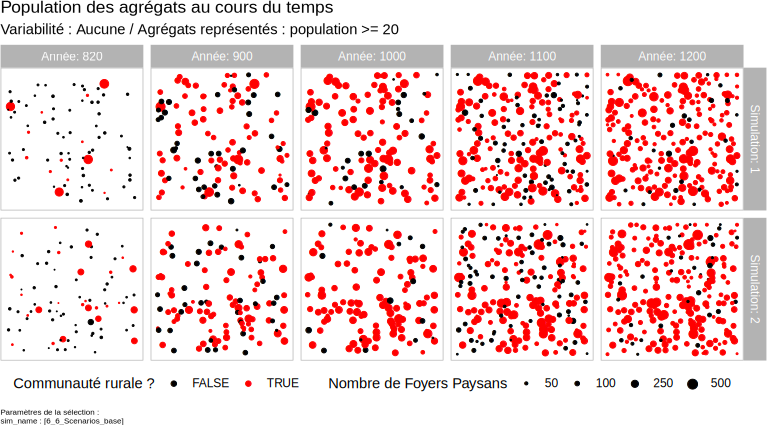
\includegraphics[width=\linewidth]{img/results_6_5_1/Agregats_Carte_Haut.pdf}
	\caption{A}
	\label{}
\end{figure}


\subsubsection{Hiérarchisation du système de peuplement}

\paragraph{Hiérarchie des agrégats}~\\


\begin{table}[H]
	\captionsetup{singlelinecheck=off}
	\centering
	\small
	{\renewcommand{\arraystretch}{1.3}%
		\begin{tabular}{p{2.5cm}|p{1.5cm}|p{1.5cm}|p{1.5cm}|p{1.5cm}|p{1.5cm}|}
			\cline{2-6}
			& \multicolumn{5}{c|}{\textbf{Nombre de foyers paysans}} \\
			  & \textbf{<100} & \textbf{101-200} & \textbf{201-300} &  \textbf{301-400} &\textbf{ >400}\\ \hline
			 \multicolumn{1}{|c|}{Nombre moyen} & 130.95 & 87.4 & 30.1 & 10.85 & 8.5 \\ \hline
			 \multicolumn{1}{|c|}{Taux moyen} & 48.8\% & 32.7\% & 11.2\% & 4.1\% & 3.2\% \\ \hline
			 \multicolumn{1}{|c|}{\textit{Objectif (taux)}} & \textit{130.95} & \textit{87.4} & \textit{30.1} & \textit{10.85} & \textit{8.5} \\ \hline	
	\end{tabular}}
	\caption{Distribution des agrégats par classe de taille en fin de simulation.}
	\label{tab:distrib-population-agregats}
\end{table}

\begin{figure}[H]
	\centering
	\includegraphics[width=\linewidth]{img/results_6_5_1/Agregats_RT_Haut.pdf}
	\caption{A}
	\label{}
\end{figure}



\paragraph{Hiérarchie des pôles}~\\

\begin{figure}[H]
	\centering
	\includegraphics[width=\linewidth]{img/results_6_5_1/Poles_RT_Haut.pdf}
	\caption{A}
	\label{}
\end{figure}
\begin{figure}[H]
	\centering
	\includegraphics[width=\linewidth]{img/results_6_5_1/Poles_Attrac_Haut.pdf}
	\caption{A}
	\label{}
\end{figure}

\paragraph{Hiérarchie des paroisses}~\\

\begin{figure}[H]
	\centering
	\includegraphics[width=\linewidth]{img/results_6_5_1/Paroisses_Compo_Haut.pdf}
	\caption{A}
	\label{}
\end{figure}
\begin{figure}[H]
	\centering
	\includegraphics[width=\linewidth]{img/results_6_5_1/Paroisses_Superficie_Haut.pdf}
	\caption{A}
	\label{}
\end{figure}


\subsubsection{Fixation et dissémination du peuplement}

\paragraph{Déplacement des foyers paysans}~\\

\begin{figure}[H]
	\centering
	\includegraphics[width=\linewidth]{img/results_6_5_1/FP_TypeDeplacements_Haut.pdf}
	\caption{A}
	\label{}
\end{figure}
\begin{figure}[H]
	\centering
	\includegraphics[width=\linewidth]{img/results_6_5_1/FP_DeplacementsDetail_Haut.pdf}
	\caption{A}
	\label{}
\end{figure}


\paragraph{Satisfaction des foyers paysans}~\\

\begin{figure}[H]
	\centering
	\includegraphics[width=\linewidth]{img/results_6_5_1/FP_Satisfaction_Haut.pdf}
	\caption{A}
	\label{}
\end{figure}
\paragraph{Nombre et dispersion des paroisses}~\\

\begin{figure}[H]
	\centering
	\includegraphics[width=\linewidth]{img/results_6_5_1/Paroisses_Nb_Haut.pdf}
	\caption{A}
	\label{}
\end{figure}

%\begin{figure}[H]
%	\centering
%	\includegraphics[width=\linewidth]{img/results_6_5_1/Poles_Nb_Haut.pdf}
%	\caption{A}
%	\label{}
%\end{figure}
\paragraph{Efficacité et équité de la desserte paroissiale}~\\



\clearpage
\section{Analyser la sensibilité de SimFeodal}

Parmi les nombreuses méthodes dédiées à l'évaluation de modèles, il en est une que l'on retrouve dans tous les manuels et dans la plupart des articles dédiés à la présentation de modèles.
Il s'agit de l'analyse de sensibilité, catégorie en fait plurielle qui regroupent l'ensemble des méthodes voués à tester ou à explorer la stabilité d'un modèle face aux éléments qui le composent : poids des \textit{inputs} dans les résultats obtenus, variabilité des résultats selon les valeurs de paramètres choisies, variabilité des résultats due à l'aléa etc.
Ces méthodes sont extrêmement nombreuses et constituent presque un champ scientifique entier, lié à l'évaluation de modèles, soient-ils à base d'agents ou statistiques.

Parmi celles-ci, les méthodes les plus classiques \autocite[257]{crooks_agent-based_2019} visent à \og déterminer l'influence des paramètres sur les sorties du modèle.\fg{} \autocite[75]{ginot2005explorer}.
Il s'agit de faire varier les valeurs des paramètres et de mesurer les écarts résultant dans les sorties.
Le plus souvent, cette mesure est quantitative, par exemple sous la forme d'un \og indice de sensibilité\fg{} qui dépend des variations des sorties mais aussi de l'amplitude de la variation des paramètres\footnote{
	Cette prise en compte de la variation des valeurs de paramètre, par exemple dans l'indice proposé par \textcite[258]{crooks_agent-based_2019} et dérivé de celui de \textcite{hamby_review_1994} (in \cite[201]{osullivan_spatial_2013}), permet de s'assurer, lors de la comparaison de la sensibilité des paramètres, que les valeurs comparées sont bien comparables.
	Pour prendre l'exemple du modèle de Schelling, il s'agit de s'assurer qu'on ne compare par une variation de 0,1\% du seuil de tolérance avec une variation de 20\% dans la part d'espace vide.
}.

Les analyses peuvent être menés en croisant des valeurs pour tous les paramètres, c'est-à-dire en analysant la sensibilité du modèle aux interactions entre paramètres.
On peut aussi procéder paramètre par paramètre, en conservant par exemple des valeurs fixes pour un jeu de paramètre (issus de calibrage) de base et en faisant varier un unique paramètre à la fois (analyse de type \textit{OFAT}, \og \textit{one factor at a time}\fg{}).

Les analyses de sensibilités sont largement recommandées comme une pratique indispensable à la validation de modèle, mais nous avons décrit dans le \hl{chapitre 3} la démarche que nous avons préféré pour l'évaluation de SimFeodal.
L'analyse de sensibilité est toutefois un outil extrêmement utile pour aider à la compréhension d'un modèle, sans chercher à en quantifier la validité.
Cette méthode repose sur l'exploration d'un modèle par le prisme de ses réactions face aux paramètres choisis, et permet ainsi de mener une étude approfondie de l'influence des paramètres.
Dans certains modèles (ref à thèse Clara), une analyse de ce type a par exemple permis de rendre plus parcimonieux un modèle KISS, en mettant en lumière le peu d'influence d'un paramètre sur l'ensemble des sorties d'un modèle.
Dans le cadre d'un modèle exploratoire, où les très nombreux paramètres comportent vraisemblablement une part de redondance, l'ambition n'est pas de réduire la masse de paramètres, mais plutôt d'aider à comprendre lesquels ont la plus grande influence sur le modèle.

Dans le cadre de SimFeodal, une analyse de sensibilité doit permettre, comme l'évaluation visuelle, de gagner en compréhension sur le modèle, et en conséquence sur les dynamiques modélisées.

La nature exploratoire et descriptive de SimFeodal rend l'application des méthodes classiques de l'analyse de sensibilité assez difficile : les paramètres ne sont pas tous quantitatifs, certains fonctionnent par paires, par grappes etc.
De manière plus générale, une analyse de sensibilité quantitative requiert à minima des objectifs quantitatifs synthétiques, hiérarchisés et parcimonieux, ce qui n'est pas la démarche empruntée dans SimFeodal.

Dans cette partie, nous nous en tiendrons à une analyse de sensibilité grossière, orientée vers une évaluation visuelle, à l'instar des autres démarches d'évaluation du modèle mises en places.
Nous nous inscrivons pleinement dans le raisonnement de \citeauteur{hirtzel2015exploration}, d'autant plus que le dit raisonnement est tenu dans une thèse dont l'analyse de sensibilité de modèles descriptifs est l'un des enjeux principaux :
\begin{quotation}
	\og Ces différents constats nous ont conduit à procéder à des analyses de sensibilité locales, avec la méthode OAT [idem \textit{OFAT}], en modifiant les valeurs de chacun des paramètres les unes après les autres, toutes choses égales par ailleurs, c’est-à-dire tous les autres paramètres étant fixés à leur valeur par défaut \textelp{}.
	Ce choix n’est pas unique dans la modélisation individu-centrée : la méthode OAT est utilisée dans plusieurs travaux en géographie ou en écologie (Ginot et al., 2006; Sanders et al., 2006; Laperrière et al., 2009; Schouten et al., 2014).
	
	Nous n’avons pas jugé indispensable le calcul d’indices de sensibilité pour étudier la sensibilité des résultats de simulation aux différents paramètres du modèle.
	Une analyse graphique à la manière de Sanders et al. (2006\st{a}), Laperrière et al. (2009) ou encore Schouten et al. (2014) nous a paru suffisante, dans un premier temps.
	Ainsi, pour reprendre les termes évoqués dans les deux sous-parties précédentes, l’analyse de sensibilité présentée dans ce chapitre est une analyse locale (OAT), avec des évaluations qualitatives de l’impact de l’incertitude émanant des valeurs de paramètres sur différents résultats de simulation.\fg{}\\
	\mbox{}~ \hfill \cite[251-252]{hirtzel2015exploration}
\end{quotation}


\subsection{Analyser la sensibilité de SimFeodal - Méthodologie}

Dans cette partie, nous décrivons et justifions brièvement la méthodologie mise en place pour l'analyse de sensibilité de SimFeodal.
Les sources informatiques, précises, de la démarche sont disponibles dans le dépôt du modèle (\hl{mettre URL dossier}).
Le détail des paramètres, les outputs du modèle, les traitements et les sorties graphiques sont disponibles quand à eux à cette adresse : \hl{depot these / anasensib}

%Mais choix d'une évaluation plutôt visuelle et qualitative, parce que paramètres très hétérogènes : liés (ex. attractivité pôle), qualitatifs (évolution besoin protection) et donc avec des étendues d'analyse de sensibilité non normalisées.
%
%+ : Résultats sur objectifs numériques uniquement, incluant contexte + émergents
%+ : Uniquement résultats du dernier pas de temps de simulation


\subsubsection{Calcul de la sensibilité}

Nous avons choisi de mener l'analyse de sensibilité de SimFeodal en empruntant l'approche \textit{OFAT}, c'est-à-dire en faisant varier les paramètres un par un.
Dans un modèle complexe où les agents sont en interactions les uns avec les autres, cette approche est forcément biaisée et lacunaire au regard d'approches plus avancées comme les méthodes d'exploration de l'espace des paramètres.
Pourtant, c'est la seule qui nous semblait applicable dans le cas de SimFeodal.
Il convient en effet de rappeler que ce modèle est caractérisé par un nombre important de paramètres : près de 70.
En ne choisissant que 5 valeurs pour chaque paramètre et pour croiser tous les paramètres, une analyse de type plan complet demanderait alors l'exécution de $5^{70} \times 20_{\text{[replications]}}$, soit environ $10^{50}$ simulations\ldots

\paragraph{Paramètres}

Dans une analyse de sensibilité, le premier choix à faire concerne les paramètres à analyser.
Dans les modèles statistiques ou KISS, l'analyse de chacun des paramètres est une évidence.
Dans des modèles plus descriptifs tels que SimFeodal (ou les modèles analysés par \textcite{hirtzel2015exploration}), on procède souvent à une sélection des paramètres afin de réduire l'ampleur de la tâche.
Par exemple, quand certains paramètres ont un ancrage empirique fort, on peut considérer qu'ils se comportent plus comme des constantes que comme des paramètres, et n'auront donc jamais à varier, et donc ne requièrent pas d'être analysés.

Dans SimFeodal, on aurait pu par exemple se passer d'analyser les paramètres de contexte les plus inscrits dans les connaissances empiriques.
Pourtant, comme nous envisageons d'éprouver le modèle sur des scénarios hétérogènes, par exemple portant sur des régions et des périodes différentes, i nous a semblé important de tester aussi ces paramètres.
On a opté pour une analyse de sensibilité de chacun des paramètres du modèle.
SimFeodal comporte dans les faits 70 paramètres, mais en pratique, le nombre de paramètres sur lesquels on peu réaliser des analyse est plus faible.
Ainsi, certains paramètres n'ont aucun sens quand mobilisés seuls.
Par exemple, deux paramètres définissent le rayon minimum et maximum des zones de prélèvement.
Il n'y a pas grand sens à faire varier l'un sans l'autre.
Dans l'analyse de sensibilité, nous considérons ces deux paramètres comme un unique paramètre à analyser, qui ne prend pas la forme d'une valeur numérique simple, mais plutôt celle d'une étendue.

Pour cette analyse de sensibilité, nous avons au final analysé 57 \og paramètres\fg{}, certains de forme numérique simple, d'autres sous formes d'étendues, et enfin quelques-uns ayant des structures plus complexes (étendues changeant au cours du temps par exemple).

\paragraph{Méthode}

La méthode choisie est simple : on définit un jeu de paramètres de base, issu du calibrage, et pour chacun des paramètres, on exécute un ensemble de simulations en faisant varier ce paramètre autour de sa valeur de base.
Comme pour toute simulation d'un modèle stochastique, il est indispensable de procéder à des réplications de ces simulations.

Comme le nombre de paramètres était déjà important, que le nombre de réplications (20) l'était lui aussi, on a choisi de mener une analyse de sensibilité assez réduite, en ne testant, pour chaque paramètre, que 5 valeurs différentes.
Ce nombre est assez faible, mais amène déjà à l'exécution de $57_{\text{[paramètres]}} \times 5_{\text{[valeurs]}} \times 20_{\text{[réplications]}} = 5700$ simulations, ce qui est une quantité importante de simulations au regard de toutes celles qui ont été mené dans les étapes de paramétrage et d'évaluation visuelle du modèle.

\paragraph{Étendue}
\label{par:etendue-parametres}

Dans une analyse de sensibilité classique, on cherche à mener des variations de paramètres comparables, c'est-à-dire centrées autour des valeurs par défaut et présentant des variations relatives de de même ampleur.
Par exemple, pour un modèle dont le premier paramètre vaut 10 et le second 100, on cherchera à répartir les valeurs testées de manière comparable : 
le premier paramètre sera testé aux valeurs 0, 5, 10, 15 et 20, et le second pour 0, 50, 100, 150 et 200.

Dans un cas réel, cette règle est difficile à suivre : on a ici pris l'exemple de paramètres quantitatifs \og de stock\fg{}, qui ne sont comparables qu'entre eux.
Dans SimFeodal, certains paramètres ont des structures bien plus difficilement comparables, à l'instar des étendues plus haut.
Comment rendre comparable cinq variations autour de 10 et cinq variations autour de l'étendue [1500m; 5000m]?
L'étendue des possibles transformations pour ces étendues est bien plus important : diminution, augmentation, translation\ldots

Ce problème se pose de manière plus importante encore pour les paramètres qui évoluent en fonction du temps.
Par exemple, le paramètre , qui agit sur la satisfaction protection des foyers paysans, a une valeur composite (de type \textit{map}, voir \cref{lst:maps-gama} dans le \hl{chapitre 2}) qui vaut \og $0$ entre 800 et 940; $0.2$ en 960 ; $0.4$ en 980 ; $0.6$ en 1000 ; $0.8$ en 1020 ; et $1$ à partir de 1040\fg{}.
Pour l'analyser dans son entièreté, il faudrait supprimer la variation en testant plusieurs valeurs, mais aussi changer le rythme de cette variation, en décaler l'étendue temporelle, en changer l'intensité etc.
Sous bien des aspects, ce paramètre peut être considéré comme qualitatif, et les variations qu'on lui appliquera dans l'analyse de sensibilité ne peuvent être que très subjectives et intrinsèquement différentes.

Face à ces difficultés, nous avons adopté une position générale acceptant la subjectivité, la non comparabilité, mais cherchant à explorer des valeurs \og caractéristiques\fg{} pour ce type de paramètres : activation et désactivation du mécanisme associé, valeur de base, et augmentation et diminution de l'ampleur de la valeur de paramètre.
Dans l'ensemble, les valeurs de paramètres choisies (\hl{mettre les tableaux en annexe}) ne sont donc que peu comparables de manière numérique, mais cela n'empêche en rien qu'elles apportent un éclairage précieux sur le comportement du modèle en fonction de ses paramètres.

\paragraph{\textit{Outputs}}

Le \hl{chapitre 5} donnait des ordres de grandeur correspondant à la masse de données produites par le modèle pour une simulation, autour de 10 Mo.
Avec 5700 simulations, un enregistrement complet des données aurait représenté plus de 50 Go de données et plus de 50 milliards de lignes de données à pré-traiter, intégrer et analyser dans la base de données.
Pour une analyse qui n'est pas au cœur de notre démarche de co-construction, cela représentait un poids bien trop important.
Nous avons donc choisi de réduire autant que possible la production d'indicateurs de sorties de simulations pour cette analyse de sensibilité.

Dans un premier temps, nous n'enregistrons l'état du modèle qu'à son pas de temps final (en 1200) plutôt que tout au long de son déroulement.
On perd certes l'aspect dynamique et la possibilité de comparer les rythmes entre les simulations, mais comme l'analyse de sensibilité doit se concentrer sur aussi peu d'objectifs que possible, ce n'est pas véritablement gênant.
Pour les mêmes raisons, on a aussi décidé de n'extraire que des données très agrégées du modèle : l'analyse de sensibilité s'appuie sur des résultats à l'échelle globale du modèle, et il n'est à ce moment nul besoin d'enregistrer les indicateurs individuels des agents du modèle.

La sélection des indicateurs agrégées a été assez rapide : on a choisit de reprendre les indicateurs numériques synthétiques, qui reprennent le tableau des objectifs présenté en \cref{tab:objectifs-types}.
Parmi ceux-ci, on a conservé uniquement les 6 indicateurs \og émergents\fg{} : 
nombre d'agrégats; nombre de grands châteaux; nombre d'églises paroissiales; distance moyenne entre églises paroissiales; part de foyers paysans isolés; augmentation de la charge fiscale
	
Dans la construction et l'évaluation du modèle, ce sont ces indicateurs que l'on a le plus observés, et s'ils n'informent pas sur l'ensemble des objectifs thématiques du modèle, ils permettent au moins de qualifier sommairement son comportement d'ensemble.

\paragraph{Computation}

Dans une analyse de sensibilité portant sur autant de simulations, la masse de données n'est pas la seule limite.
Le temps de calcul l'est tout autant, sinon plus, tant il peut s'étendre rapidement.
Sur un ordinateur individuel, avec les valeurs de paramètre décidées après calibrage, chaque simulation demande en moyenne 5 minutes de calcul.
Multiplié par les 5700 simulations requises, l'exécution des simulations nécessaires à l'analyse de sensibilité réclame alors un temps de calcul de près de 20 jours sur un ordinateur individuel, sans véritable droit à l'erreur sous faute de recommencer ce quasi-mois de calcul.

Pour que cette analyse soit effectuée dans un délai plus raisonnable, nous avons utilisé les capacités de calcul d'un serveur du laboratoire ainsi que d'un serveur de calcul géré par la TGIR Huma-Num.
En distribuant les exécutions de simulation sur la quarantaine de processeurs informatiques que cela représentait au total, tout en laissant tourner les simulations uniquement de nuit pour ne pas gêner les autres utilisateurs de ces serveurs, toutes les simulations requises ont été exécutées en 3 jours, ce qui représente cette fois-ci un investissement temporel bien plus raisonnable.

\subsubsection{Analyse Quantitative - Filtrage des paramètres}

Devant la masse de paramètres à analyser, nous avons réalisé qu'il était difficile de mener une analyse visuelle directe de la sensibilité des paramètres.
Il a donc été choisi de mener une première étape, quantitative, pour permettre de trier et de filtrer un sous-ensemble de paramètres dont une étude plus approfondie serait alors possible.

Pour cette étape, on a raisonné à l'échelle agrégée du paramètre, en cherchant à mesurer la variabilité des indicateurs de sortie choisis provoquée par la variation des valeurs de paramètres.

\paragraph{Normalisation des objectifs}

Un premier problème est que les indicateurs de sortie de simulation choisis, les objectifs, sont très hétérogènes en termes d'ordre de grandeur.
Il était donc nécessaire de procéder à un \og centrage\fg{} des données issues de la simulation.
Ce centrage peut être effectué, classiquement, sur les valeurs obtenues, pour obtenir une moyenne valant 0, comme on le fait lors d'une normalisation classique de données.

Pour l'étude de SimFeodal, nous avons préféré centrer les données de chaque indicateur relativement aux objectifs numériques identifiés.
Par exemple, une simulation produisant 250 agrégats, quand l'objectif numérique est de 200, aura pour indicateur \og nombre d'agrégats\fg{} 50.
Cela permet de mesurer les comportements de manière plus thématique qu'un centrage statistique autour de 0.
Pour chaque indicateur, on a donc soustrait à la valeur obtenue par simulation la \og valeur attendue\fg{}, identifiée thématiquement comme objectif (voir le \cref{tab:results-basique}).
Après cela, pour chaque indicateur pris individuellement, les données générées par chaque simulation deviennent comparables.

Pour atteindre une comparabilité plus importante entre des données hétérogènes, on procède aussi usuellement à une \og réduction\fg{} des données, c'est-à-dire à la normalisation de leur variabilité (écart-type).
Classiquement, cette étape consiste à diviser chaque résultat par l'écart-type.
On obtient ainsi, pour chaque série de donnée, un écart-type de 1, qui permet alors de comparer la variabilité de ces séries hétérogènes.
Comme pour le centrage, on a choisi de réduire les données en fonction de données connues plutôt qu'autour d'une valeur abstraire de 1.
On a préféré pour cela se référer à nos données simulées de référence, c'est-à-dire issues des simulations présentées dans la première partie de ce chapitre, après calibrage.
Les données centrées ont ainsi été ensuite divisées par l'écart-type mesuré sur les simulations de cette version de référence, pour chaque indicateur numérique.

Au final, ce procédé de normalisation est très proche d'une normalisation statistique classique, mais se base sur des valeurs qui ont un sens dans le modèle plutôt que sur les valeurs \og abstraites\fg{} que constituent une moyenne à 0 et un écart-type de 1.

\vspace{-2em}\begin{flalign*}
& \text{valeur\_normalis\'ee}_{\text{indicateur\_i}} = & 
\frac{
 	\text{valeur}_{\text{indicateur\_i}} - \text{valeur\_attendue}_{\text{indicateur\_i}}
 }{
 \sigma(\text{valeurs\_calibr\'ees}_\text{{indicateur\_i}})
} &
\end{flalign*}

Ainsi conçue, la valeur normalisée permet une comparabilité au sein des indicateurs, mais aussi entre eux puisque les ordres de grandeur sont désormais similaires.

\paragraph{Calcul de la sensibilité}

Comme les valeurs sont désormais normalisées, il est possible de mener des opération conjointes sur les différents indicateurs.
On définit un indice global, intitulé \og sensibilité\fg{}, qui correspond à une moyenne, pour chaque paramètre, de ses valeurs normalisées dans chacun des indicateurs.
Après le centrage, les valeurs deviennent négatives ou positives selon qu'elles sont inférieures ou supérieures aux objectifs.
Pour un paramètre qui verrait des variations importantes, négatives et positives, le risque d'une moyenne est alors que la sensibilité calculée soit faible, le très positif compensant le très négatif.
Pour prévenir ce risque, on a choisi de calculer la sensibilité sur les valeurs absolues des valeurs normalisées plutôt que sur leur valeur brut.
La sensibilité de chaque paramètre peut alors être définie comme suit :

\vspace{-2em}\begin{flalign*}
& \text{sensibilit\'e}_{\text{param\`etre}\_\upalpha} = \\
& \frac{1}{n_{\text{indicateurs}}
	\times n_{\text{valeurs\_param\`etres}\_\upalpha}
	\times n_{\text{r\'eplications}}}
\sum |\text{valeurs\_normalis\'ees}_{\text{param\`etre}\_\upalpha}|
\end{flalign*}

\paragraph{Sélection de paramètres}

En calculant la sensibilité de chaque paramètre, on sera en mesure d'en sélectionner un sous-ensemble afin de procéder à une analyse visuelle de la sensibilité de ces derniers.
Pour isoler ce sous-ensemble, on ne conservera que les paramètres à la plus forte sensibilité globale, en cherchant à en conserver une dizaine.
Ce nombre est volontairement imprécis puisqu'il dépendra surtout de la forme de la distribution de la sensibilité des paramètres : on cherchera avant tout à isoler des paramètres dont la sensibilité les différencie franchement des autres.
On se basera pour cela sur une méthode entièrement subjective d'examen visuel des écarts entre les valeurs de sensibilité, tel qu'on peut le faire pour choisir un nombre de classes à étudier lors de l'exécution d'une classification ascendante hiérarchique.

Un risque de cette méthode est que certains indicateurs peuvent contribuer bien davantage que d'autres à la sensibilité d'ensemble, malgré la normalisation.
Pour ne pas risquer de négliger des paramètres dont la sensibilité s'exprimerait uniquement sur certains indicateurs, on complètera la sélection de paramètres précédente par une sélection des trois paramètres les plus sensibles sur chacun des 6 indicateurs.

\vspace{-2em}\begin{flalign*}
& \text{sensibilit\'e}_{\text{param\`etre}\_\upalpha_{\text{indicateur\_i}}} = \\
& \frac{1}{n_{\text{valeurs\_param\`etres}\_\upalpha}
	\times n_{\text{r\'eplications}}}
\sum |\text{valeurs\_normalis\'ees}_{\text{param\`etre}\_\upalpha_{\text{indicateur\_i}}}|
\end{flalign*}


En considérant qu'une large partie de ces paramètres auront vraisemblablement déjà été isolés par le filtre sur la sensibilité globale, on devrait obtenir quelques paramètres supplémentaires sur lesquels mener l'analyse visuelle.

\subsubsection{Analyse visuelle}

Une fois les paramètres à étudier sélectionnés, on pourra alors mener une analyse visuelle pour comprendre l'influence des paramètres sur les indicateurs de sortie du modèle.
Le nombre de paramètres étant réduit, il sera possible d'analyser l'importance de cette influence (la sensibilité), mais aussi sa cardinalité : en observant la réaction des indicateurs de sortie en fonction des valeurs de paramètre, on
pourra noter les corrélations (visuelles).

Cette analyse visuelle de sensibilité s'inscrit ainsi dans une analyse à la fois technique et thématique de SimFeodal.
Elle doit en effet permettre de gagner en compréhension sur les interactions entre paramètres et mécanismes.
Cela devrait éclairer l'aspect technique, lié à la validation interne du modèle -- tel paramètre que l'on pense jouer sur tel mécanisme se comporte-t-il bien comme attendu ? -- et l'aspect thématique -- est-ce que la taille du monde simulé a 


\paragraph{Visualisation}

L'objectif de la visualisation de la variation des paramètres est d'observer, pour chaque paramètre, comment ce dernier varie sur chacun des indicateurs.
Pour cela, on représente donc la variation due aux réplications de chaque paramètre au moyen de représentations visuelles dédiées à la variabilité, comme des \textit{box-plots} ou \textit{violin-plots}.
La \cref{fig:exemple-visu-sensib} présente un exemple de mise en page de telles représentations graphiques afin de faciliter l'analyse de sensibilité visuelle.
\begin{figure}[H]
	\centering
	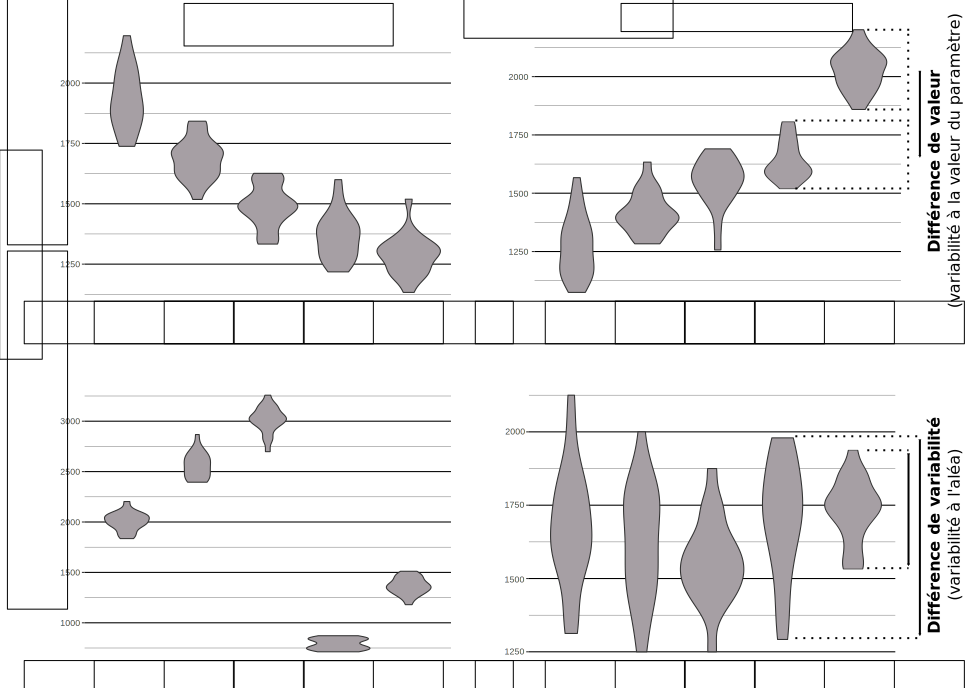
\includegraphics[width=.9\linewidth]{img/schema_violinplots_sensib.pdf}
	\caption{Construction et mise en page de planches graphiques dédiés à l'analyse visuelle de la sensibilité des 5 modalités de $\upomega$ paramètres sur \textit{n} indicateurs.}
	\label{fig:exemple-visu-sensib}
\end{figure}

\paragraph{Normalisation}

La normalisation des valeurs afin d'homogénéiser indicateurs et variation des paramètres était indispensable afin de garantir une comparabilité acceptable lors de l'analyse de l'ensemble des paramètres.
Pourtant, sur un sous-ensemble de paramètres qui doivent être étudiés plus précisément, cette normalisation est un frein à l'interprétation : les valeurs des différents indicateurs ne sont plus exprimés dans l'unité d'origine et il est alors difficile d'en faire un commentaire thématique.
L'analyse visuelle sera ainsi présentée sur les valeurs brutes issues des simulations, et chaque graphique aura en conséquence un axe des ordonnées propre.

\subsection{Sélection des paramètres}

\begin{figure}[H]
	\centering
	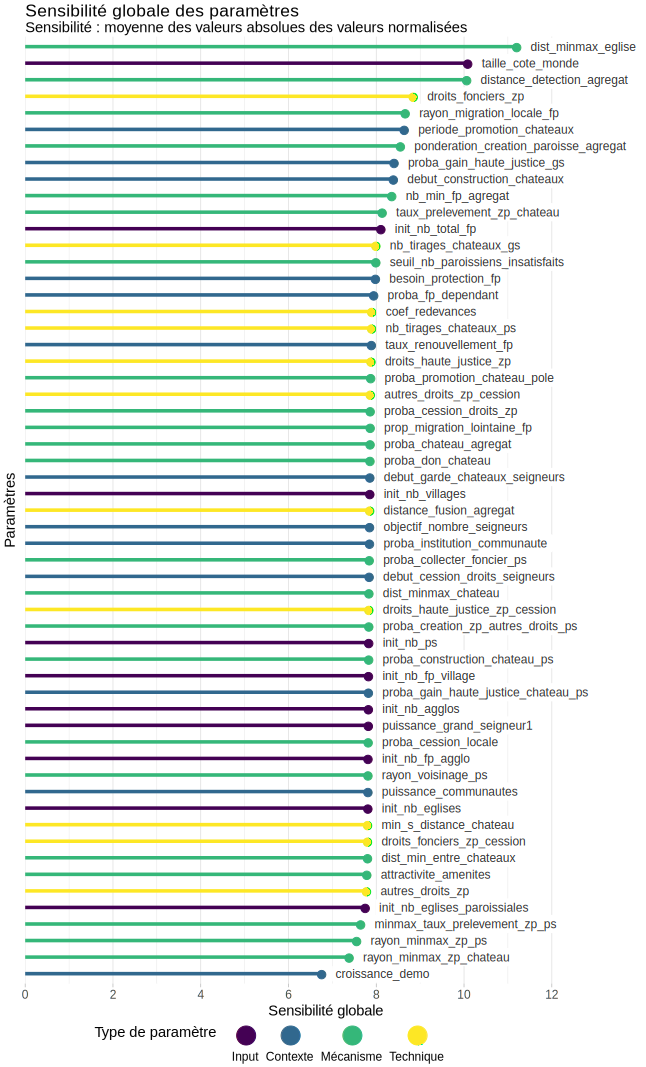
\includegraphics[width=\linewidth]{img/sensibilite_globale.pdf}
	\caption{Analyse de la sensibilité d'ensemble de tous les paramètres de SimFeodal.}
	\label{fig:sensibilite-globale}
\end{figure}

La \cref{fig:sensibilite-globale} présente les \og scores de sensibilité\fg{} de chacun des paramètres du modèle.

Une première remarque est que de manière légèrement contre-intuitive, on ne peut discerner de motif particulier selon les types de paramètres : les \textit{inputs}, paramètres de contexte, de mécanisme et enfin les paramètres techniques sont dispersés et entremêlés dans le graphique.
On se serait vraisemblablement attendu à ce que les inputs et paramètres de contexte jouent un rôle plus important que les paramètres techniques par exemple.

Pondérons toutefois cette remarque en rappelant que malgré une homogénéisation des valeurs en sortie par leur normalisation, il n'y a ici aucune compensation de l'étendue très variable des valeurs de paramètre testées (\hl{disponibles dans l'annexe N}).
Par exemple, si l'on compare un paramètre très sensible (la taille du monde simulé, \textsf{taille\_cote\_monde}) et un paramètre peu sensible (le taux de croissance démographique introduit dans le modèle, \textsf{croissance\_demo}), on peut réaliser que l'ordre de grandeur de la variation est faible.
\begin{itemize}[noitemsep,nolistsep]\vspace*{-.5em}
	\item Pour \textsf{taille\_cote\_monde}, dont la valeur de base est de 80 km, les valeurs testées sont 50, 75, 100, 125 et 150 km.
	Il y a donc à peu près une variation qui va de la moitié de la valeur de base à son double.
	\item Pour \textsf{croissance\_demo}, les seuils sont plus restreints.
	Pour ne pas déstabiliser les autres indicateurs, ce paramètre a été modifié en tenant compte d'une population finale stable de 40 000 foyers paysans, en adaptant donc à chaque valeur de croissance démographique une valeur différente de population initiale.
	De ce fait, la valeur de base de croissance démographique est de 0\%, et les valeurs testées sont de 1.53\%, 3.72\%, 5.89\% et 12.89\%.
	Ces valeurs permettent de faire passer la population de la stabilité au décuplement. Au regard du paramètre précédent, l'étendue interprétée est large, mais en absolu, les 4 premières valeurs sont très proches et on ne s'attend ainsi pas à ce qu'elles aient un effet majeur sur les sorties du modèle.
\end{itemize}

Un autre exemple de ces étendues incomparables permet d'éclairer la première remarque quant au fait que les paramètres techniques ne sont pas relégués en bas de ce graphique.
Par définition, les paramètres techniques ont des valeurs qui ne représentent strictement rien d'un point de vue thématique.
Leur étendue acceptable est alors extrêmement difficile à évaluer, et on aura ainsi pu avoir tendance à effectuer de mauvais jugements sur les valeurs testées de ces paramètres, les conduisant soit à être sur-valués (le paramètre de caractérisation des droits fonciers, \textsf{droits\_fonciers\_zp} semble entrer dans cette catégorie avant examen spécifique), soit à sembler sous-valués (le paramètre \textsf{distance\_fusion\_agregat} par exemple, a été modifié à de nombreuses reprises lors du paramétrage du modèle et était à ce moment assez important).

Notons aussi que dans les 10 paramètres jugés les plus sensibles, 4 portent sur des valeurs testés \og qualitatives\fg{} (étendues, variables au cours du temps\ldots, voir p.~\pageref{par:etendue-parametres}), alors que ces paramètres ne représentent que 20\% de l'ensemble des paramètres testés.
Là encore, on peut estimer que cette légère sur-représentation de ces paramètres est à la difficulté de leur attribuer des étendues comparables.

Un dernier constat, à l'échelle très agrégée qui caractérise ces analyses, nous paraît extrêmement rassurant en termes de validation interne du modèle : aucun des paramètres testés ne présente une sensibilité véritablement faible, qui plus est en considérant que la plus faible sensibilité mesurée (paramètre \textsf{croissance\_demo}) correspond à un paramètre dont l'on sait qu'il a une influence réelle sur les sorties du modèle.
Ce simple constat nous indique que dans la limite du jeu de paramètre issu du calibrage, aucun paramètre n'est inutile, et ne devrait par conséquent être supprimé du modèle si on recherchait une parcimonie plus importante à cette étape.



À la lecture du graphique, on remarque qu'autour des 10 premiers paramètres, on peut constater qu'un \og saut\fg{} dans les valeurs de sensibilité se produit entre les paramètres \textsf{nb\_min\_fp\_agregat} et \textsf{taux\_prelevement\_zp\_chateau}.
L'écart entre ce dernier paramètre et le suivant est en effet assez faible, et on décide de ne conserver que les 10 premières paramètres (le 10ème est \textsf{nb\_min\_fp\_agregat}) pour l'analyse visuelle.

La sélection des trois paramètres ayant la plus forte sensibilité sur chaque indicateur complète cette liste avec 4 nouveaux paramètres, portant donc le total à 14 paramètres dont la sensibilité sera analysée visuellement.
Le \cref{tab:selection-parametres-anavis} en présente la liste.

\begin{table}[H]
	\captionsetup{singlelinecheck=off}
	\centering
	{\renewcommand{\arraystretch}{1.3}%
	\begin{tabular}{|p{7cm}|p{5.25cm}|m{1.25cm}|}
	\hline
\textbf{Paramètre} & \textbf{Origine de la sélection} & \textbf{Rang sensibilité} \\ \hline
dist\_minmax\_eglise & Globale & 1 \\ \hline
taille\_cote\_monde & Globale & 2 \\ \hline
distance\_detection\_agregat & Globale & 3 \\ \hline
droits\_fonciers\_zp & Globale & 4 \\ \hline
rayon\_migration\_locale\_fp & Globale & 5 \\ \hline
periode\_promotion\_chateaux & Globale & 6 \\ \hline
ponderation\_creation\_paroisse\_agregat & Globale & 7 \\ \hline
proba\_gain\_haute\_justice\_gs & Globale & 8 \\ \hline
debut\_construction\_chateaux & Globale & 9 \\ \hline
nb\_min\_fp\_agregat & Globale & 10 \\ \hline
taux\_prelevement\_zp\_chateau & ratio\_charge\_fiscale & 11 \\ \hline
nb\_tirages\_chateaux\_ps & nb\_grands\_chateaux & 18 \\ \hline			
proba\_creation\_zp\_autres\_droits\_ps & distance\_eglises\_paroissiales & 36 \\ \hline
croissance\_demo & ratio\_charge\_fiscale & 57 \\ \hline
\end{tabular}}
\caption[Paramètres sélectionnés pour l'analyse visuelle.]{Paramètres sélectionnés pour l'analyse visuelle.\\
	\textit{La colonne d'origine indique si les paramètres ont été sélectionnés selon leur score de sensibilité global, ou sinon, l'indicateur qu'ils affectaient particulièrement.}}
\label{tab:selection-parametres-anavis}
\end{table}


\end{figure}


\section{Analyser la sensibilité de SimFeodal}
\subsection{Analyse de sensibilité - Méthodo}
\subsection{Analyse de sensibilité - Résultats (quanti))}
\subsection{Analyse de sensibilité - Évaluation visuelle}
\subsection{Analyser la sensibilité à l'aléa}

\section{Comprendre le modèle par l'exécution de scénarios}
\subsection{Tester l'hypothèse d'une croissance démographique}
\subsection{Modéliser la dépendance spatiale : le poids du servage}
\subsection{Quel rôle et importance des communautés paysannes dans la structuration du système de peuplement ?}